\chapter{Spreading} % (fold)
\label{cha:spreading}

\section{Which model for news spreading?}

In order to choose a model for the spreading of news or ideas it's necessary to point out
what means in this field an infection, and to interpret the related quantities.
A person "infected'' by a news it's not a person just only reached by the news, but it's a person
who partecipates to the spreading by communicating to its neighbours and potentially infect them.
The decision to spread the information it's an individual choice, expressing the interest
of the person to the news, and indicates the presence of a personal threshold of reaction related to the news or ideas.
The threshold can also be influenced by the neighbourhood or the community membership.


In the epidemic models, such as the SI model, the coefficient $\beta$ represents the rate of trasmission of the infection and it is constant for the whole population, indicating the dependence on the properties of the pathogen.

In the news field $\beta$ can be interpreted as an intrinsic power of trasmission of the news.
This power of trasmission may be associated to the journalistic concept of \textit{newsworthiness},
which includes all the characteristics that make a fact a worthy news.
But the expanding phenomenon of \textit{fake news} shows that the speed of diffusion it's not only related to
the worthiness of an information. A recent paper published on Science \cite{Vosoughi_2018} shows how false news on Twitter spread 
``significantly farther, faster, deeper, and more broadly than the truth in all categories of information''.
The authors of the paper tried to explain the faster speed of diffusion of the false news by its novelty and the conveying
of strongest emotive reactions like surprise or disgust.


A news coverage is usually characterized also by a certain amount of time after which the news naturally ``dies'' out.
This fact can be modeled with the SIS formulation where the people recover from the infection with a rate $\mu$.
The coefficient $\mu$, likewise $\beta$, it's constant and in this case can represents the intrinsic property of a news to vanish,
which makes the people stopping communicating about the news.


In order to include also the personal threshold reaction to a news would be necessary to use a more sophisticated model, MILLI

In this chapter we'll describe the results we obtained by applying the \textbf{SI}, \textbf{SIS}, \textbf{SIR},
and \textbf{Threshold} diffusion models both on the crawled data and on the synthetic graphs (Erdős–Rényi and
Barabási–Albert) generated from the original one. In each section, a comparison between the three networks will be
provided along with some details on the implementation of the tests of every model.


\section{The New York Times vs La Repubblica }

Idea: let's start with the same news, but two different nodes, there is a big difference in diffusion?
Prevision: no, the difference it's minimal because of the presence of hubs.








\section{SI model} % (fold)
\label{sec:si_model}
    \begin{figure}[H]
        \centering
        \begin{subfigure}{0.45\textwidth}
            \resizebox{\textwidth}{!}{
                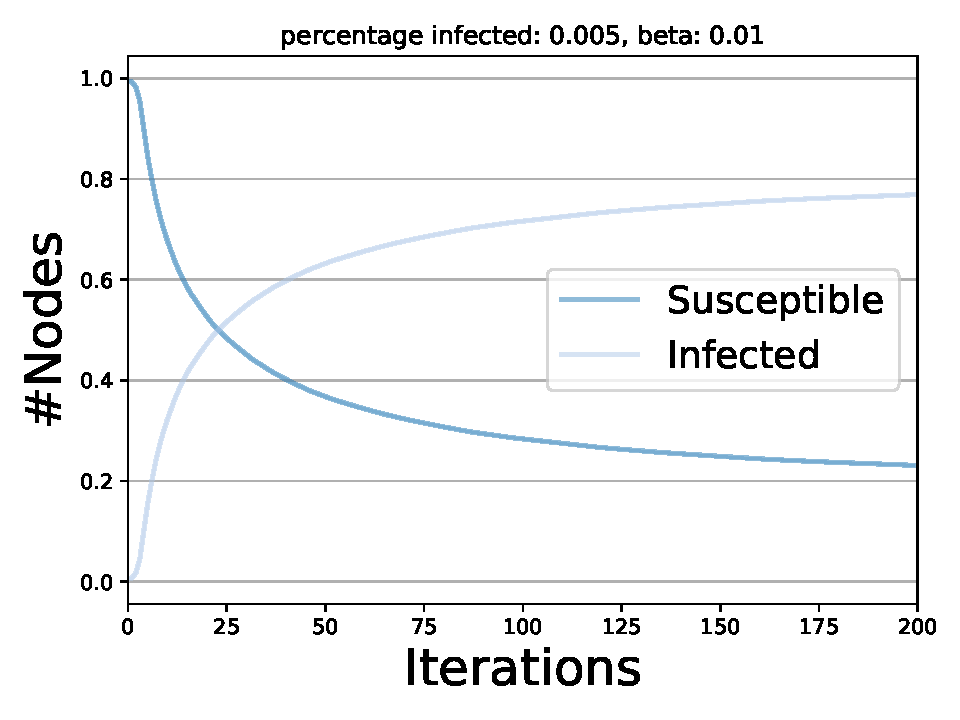
\includegraphics{images/spreading/si/diffusion.pdf}

            }
            \caption{}
            \label{diff_si}
        \end{subfigure}
        \begin{subfigure}{0.45\textwidth}
            \resizebox{\textwidth}{!}{
                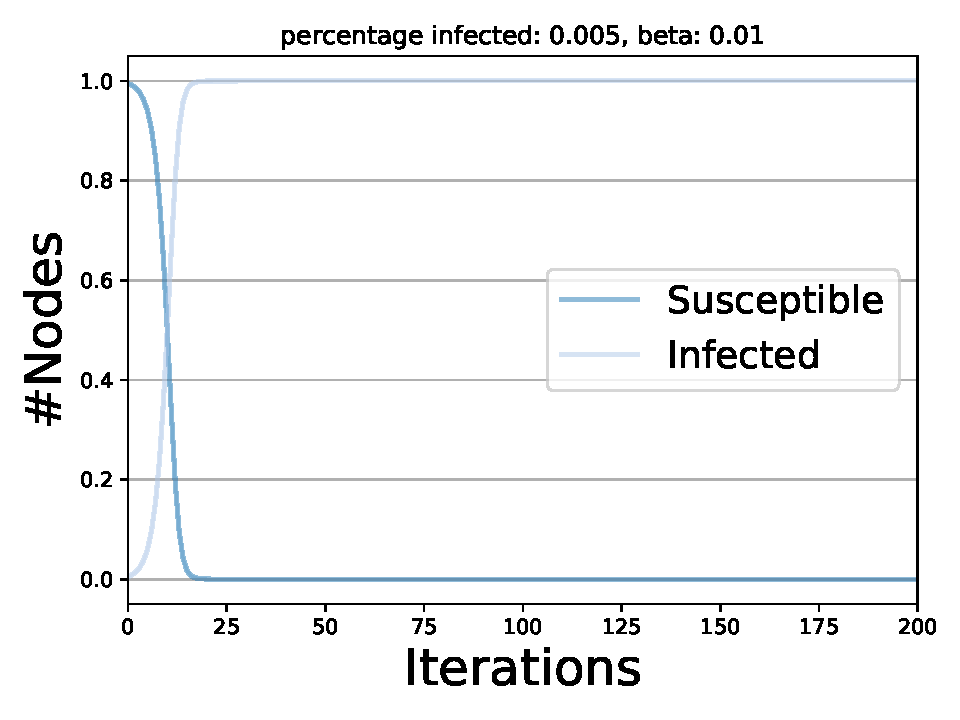
\includegraphics{images/spreading/si/diffusion_er.pdf}
            }
            \caption{}
            \label{diff_si_er}
        \end{subfigure}
        \begin{subfigure}{0.45\textwidth}
            \resizebox{\textwidth}{!}{
                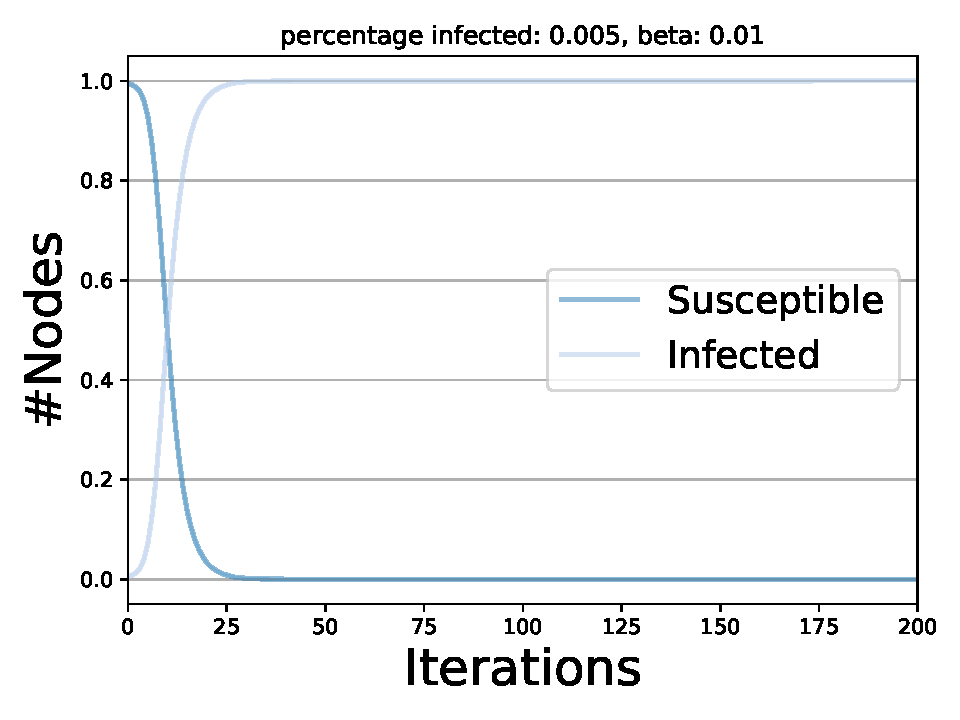
\includegraphics{images/spreading/si/diffusion_ba.pdf}
            }
            \caption{}
            \label{diff_si_ba}
        \end{subfigure}
        \begin{subfigure}{0.45\textwidth}
            \resizebox{\textwidth}{!}{
                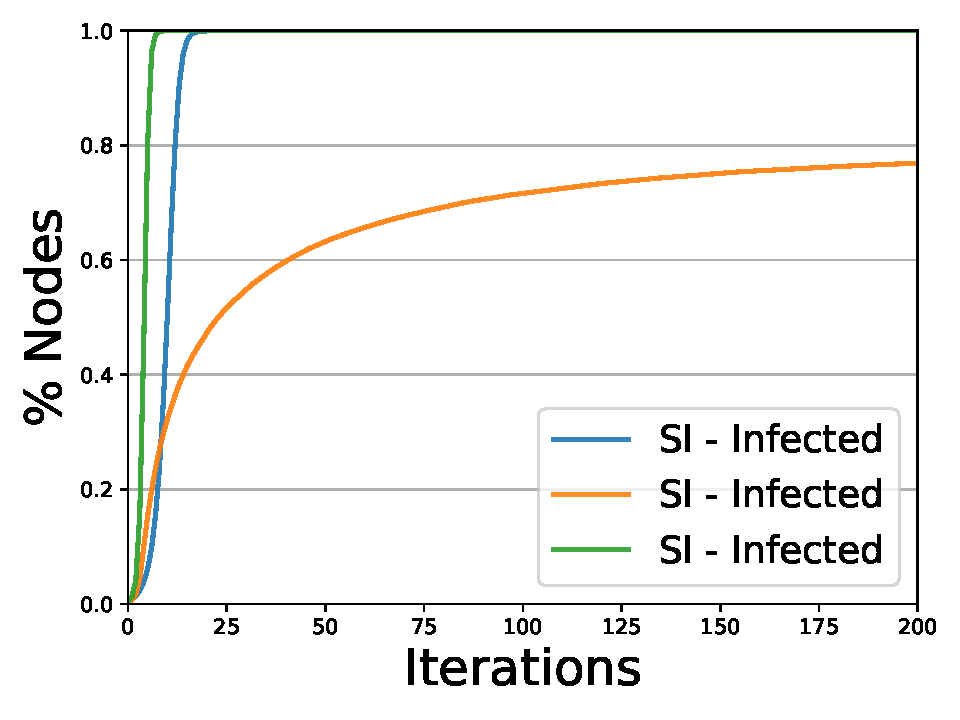
\includegraphics{images/spreading/si/trend_comparison.pdf}
            }
            \caption{}
            \label{diff_si_comparison}
        \end{subfigure}
        \caption{In Figure \ref{diff_si} we can see the diffusion graph for the original network, while in Figure
        \ref{diff_si_er} and in Figure \ref{diff_si_ba} we can see the diffusion graph for the Erdős–Rényi and
        Barabási–Albert networks, respectively. In Figure \ref{diff_si_comparison} we can see a comparison between
        the infection rate of the three networks.}
        \label{diff_si_total}
    \end{figure}
    For the \textbf{Susceptible-Infected} model we've started with a $0.005\%$ of the total population ($3$ nodes)
    of each network being infected, and we've choosed a value of $0.01$ for the infection rate $\beta$. As you can
    see from Figure \ref{diff_si_total}, the original network is the only one that doesn't reach the saturation
    regime, while the other networks reach it within the first $25$ iterations of the model. This is due to the fact
    that both the Erdős–Rényi and the Barabási–Albert network are extremely connected, hence it is more easy for the
    infection to spread among the nodes.

% section si_model (end)

\section{SIS model} % (fold)
\label{sec:sis_model}
    \begin{figure}[H]
        \centering
        \begin{subfigure}{0.45\textwidth}
            \resizebox{\textwidth}{!}{
                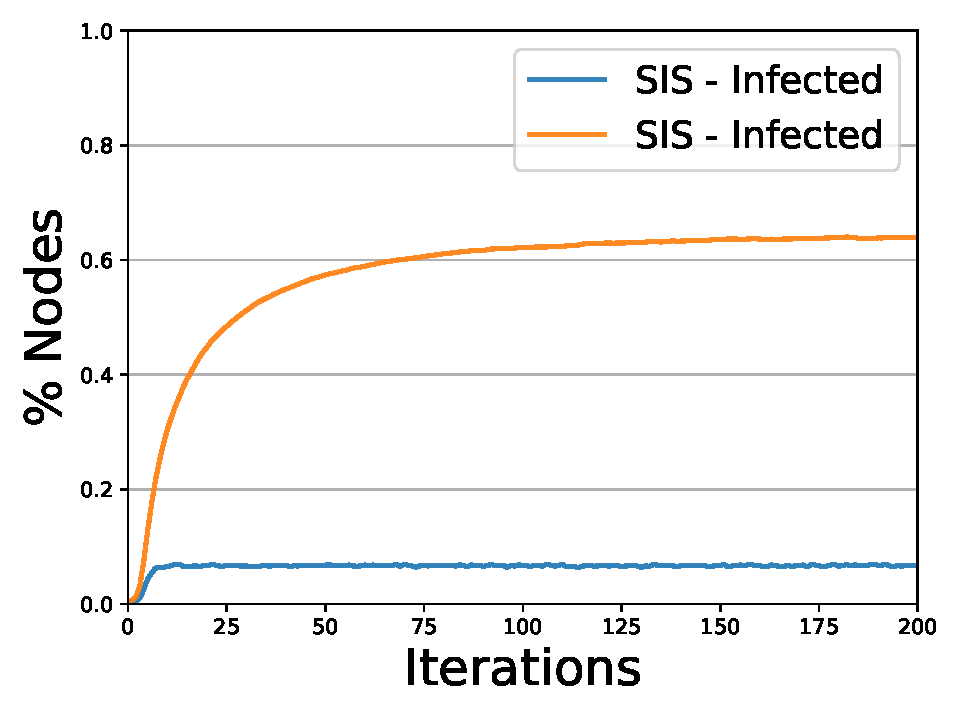
\includegraphics{images/spreading/sis/diffusion_original_comparison.pdf}
            }
            \caption{}
            \label{diff_sis}
        \end{subfigure}
        \begin{subfigure}{0.45\textwidth}
            \resizebox{\textwidth}{!}{
                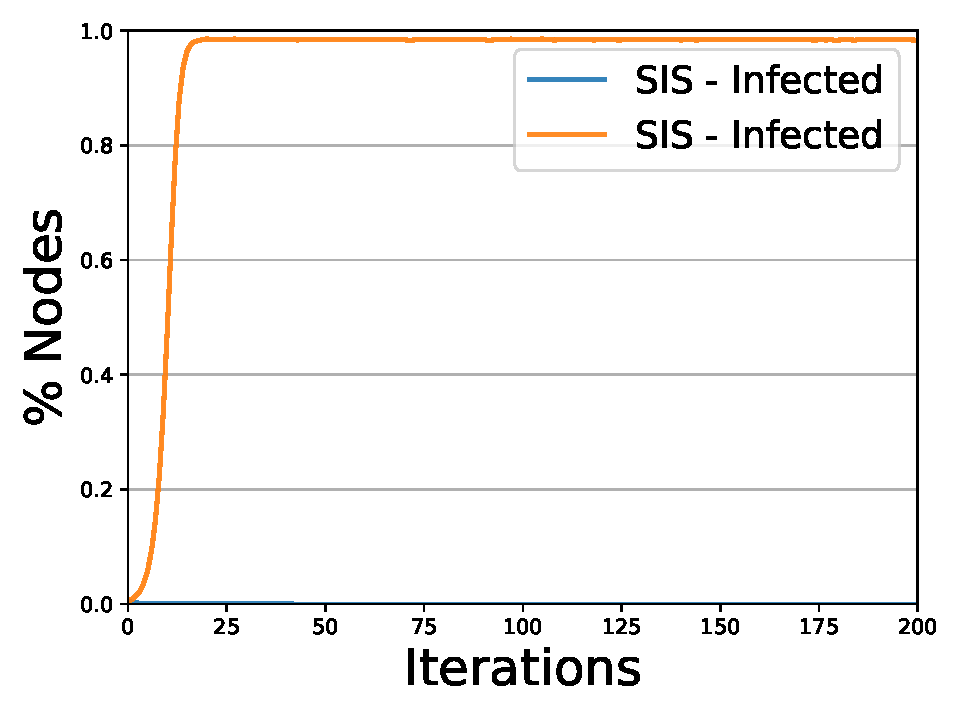
\includegraphics{images/spreading/sis/diffusion_er_comparison.pdf}
            }
            \caption{}
            \label{diff_sis_er}
        \end{subfigure}
        \begin{subfigure}{0.45\textwidth}
            \resizebox{\textwidth}{!}{
                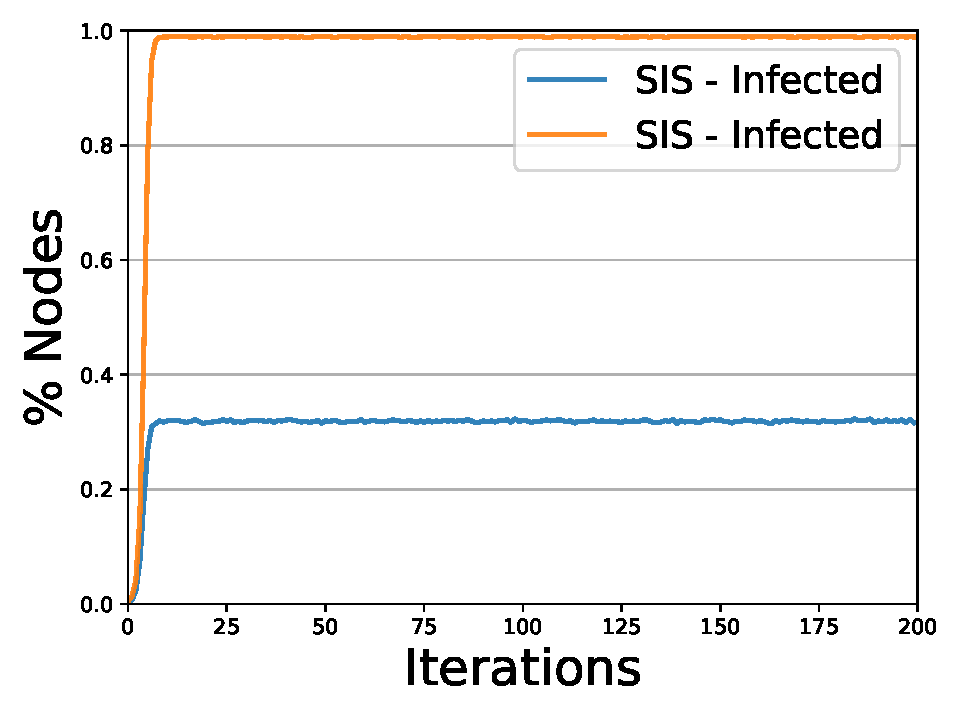
\includegraphics{images/spreading/sis/diffusion_ba_comparison.pdf}
            }
            \caption{}
            \label{diff_sis_ba}
        \end{subfigure}
        \caption{In Figure \ref{diff_sis} we can see the comparison between the endemic state, in orange, and the
        disease free state, in blue, for the original network. The same comparison can be observed for the
        Erdős–Rényi and the Barabási–Albert network, respectively, in Figure \ref{diff_sis_er} and
        \ref{diff_sis_ba}}
        \label{diff_sis_total}
    \end{figure}
    For the \textbf{Susceptible-Infected-Susceptible} model, thanks to the introduction of the recovery rate $\mu$,
    we can model two possible outcomes for the epidemic: the \textbf{endemic state}, characterized by a low recovery
    rate and by the fraction of infected individuals that follows a logistic curve similar to the one observed for
    the SI model, for which $\mu < \beta\langle k \rangle$, and the \textbf{disease free} state, characterized by a
    sufficiently high recovery rate, for which $\mu > \beta\langle k \rangle$. A comparison between this two states
    is represented for every network in Figure \ref{diff_sis_total}.

% section sis_model (end)

\section{SIR model} % (fold){}
\label{sec:sir_model}
    The key characteristic of the \textbf{Susceptible-Infected-Recovered} model consist in introducing the
    probability $\gamma$ for the individuals to recover from the disease and hence to be "removed" from the
    population instead of returning to the susceptible state. We have choosen to test this model either for the case
    in which $\gamma$ is smaller than $\beta$ and the other way around. The graphs representing this different
    situations for all the three networks are visible in Figure \ref{diff_sir_total}.
    \begin{figure}
        \begin{subfigure}{0.33\textwidth}
            \resizebox{\textwidth}{!}{
                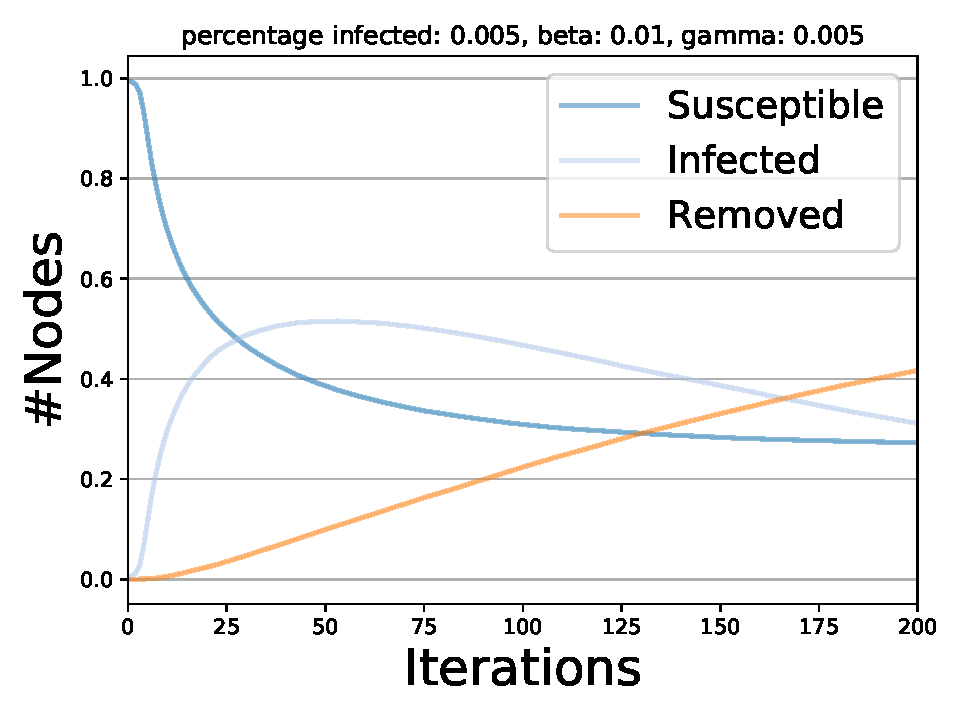
\includegraphics{images/spreading/sir/diffusion_smaller.pdf}
            }
            \caption{}
            \label{diff_sir_smaller}
        \end{subfigure}
        \begin{subfigure}{0.33\textwidth}
            \resizebox{\textwidth}{!}{
                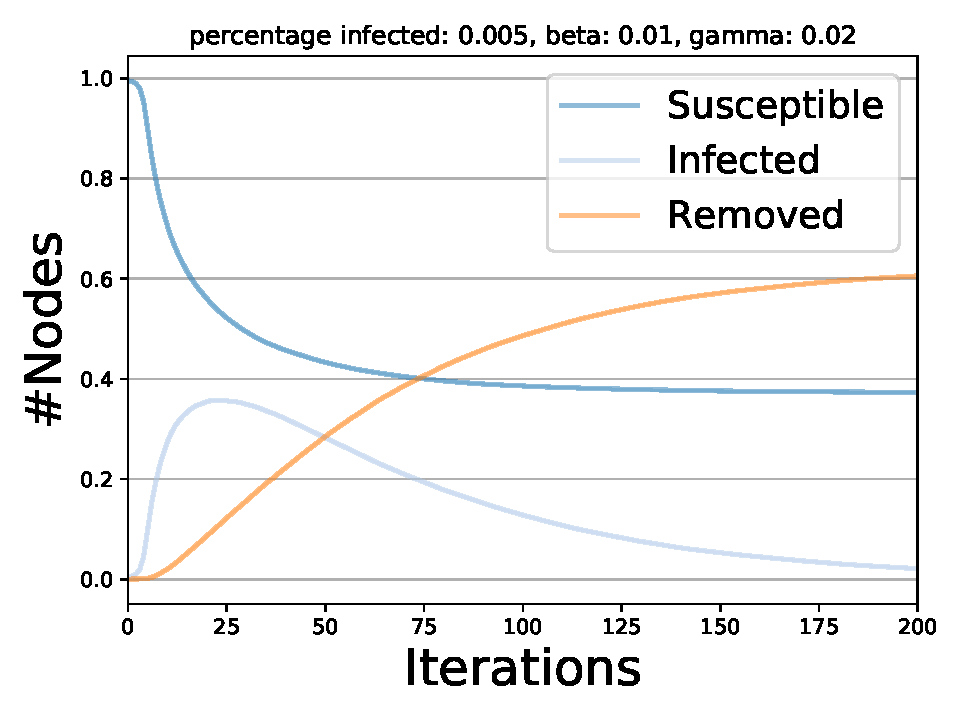
\includegraphics{images/spreading/sir/diffusion_greater.pdf}
            }
            \caption{}
            \label{diff_sir_greater}
        \end{subfigure}
        \begin{subfigure}{0.33\textwidth}
            \resizebox{\textwidth}{!}{
                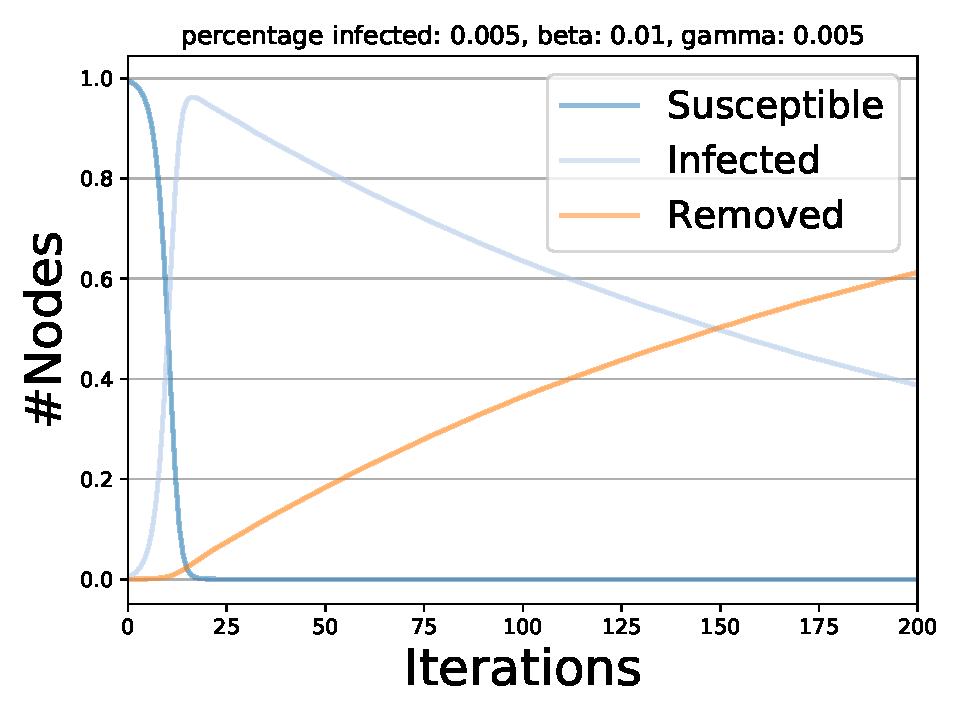
\includegraphics{images/spreading/sir/diffusion_er_smaller.pdf}
            }
            \caption{}
            \label{diff_sir_er_smaller}
        \end{subfigure}
        \begin{subfigure}{0.33\textwidth}
            \resizebox{\textwidth}{!}{
                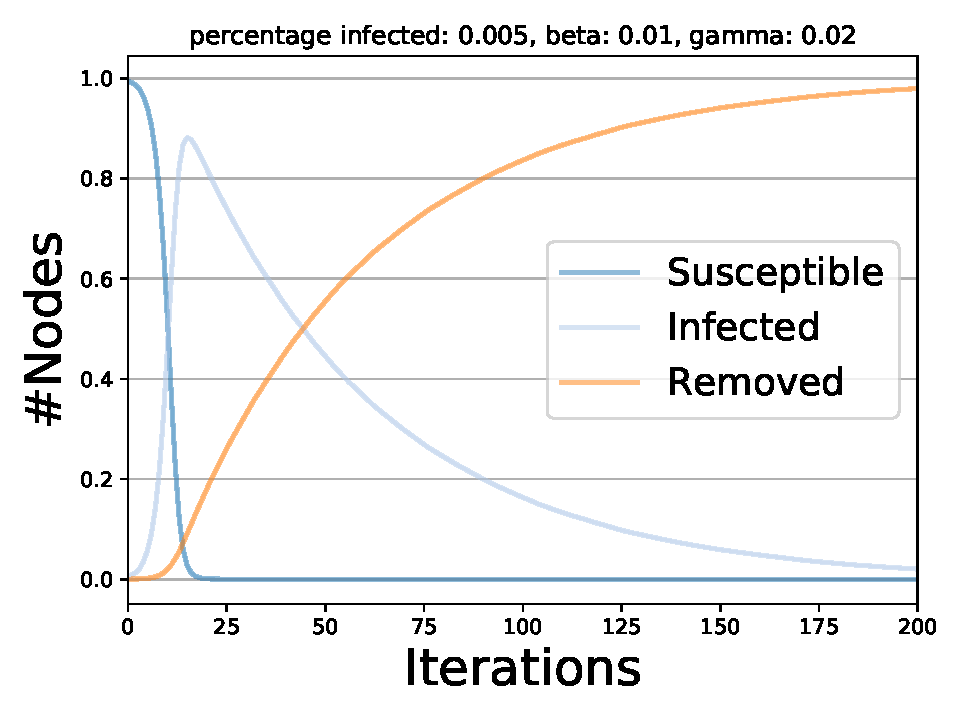
\includegraphics{images/spreading/sir/diffusion_er_greater.pdf}
            }
            \caption{}
            \label{diff_sir_er_greater}
        \end{subfigure}
        \begin{subfigure}{0.33\textwidth}
            \resizebox{\textwidth}{!}{
                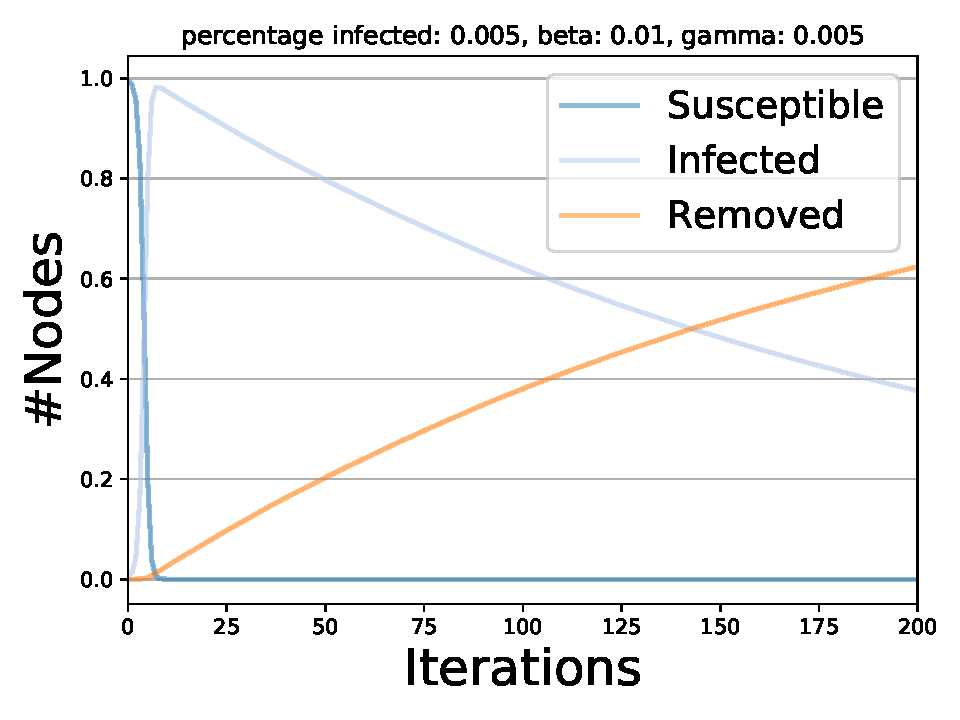
\includegraphics{images/spreading/sir/diffusion_ba_smaller.pdf}
            }
            \caption{}
            \label{diff_sir_ba_smaller}
        \end{subfigure}
        \begin{subfigure}{0.33\textwidth}
            \resizebox{\textwidth}{!}{
                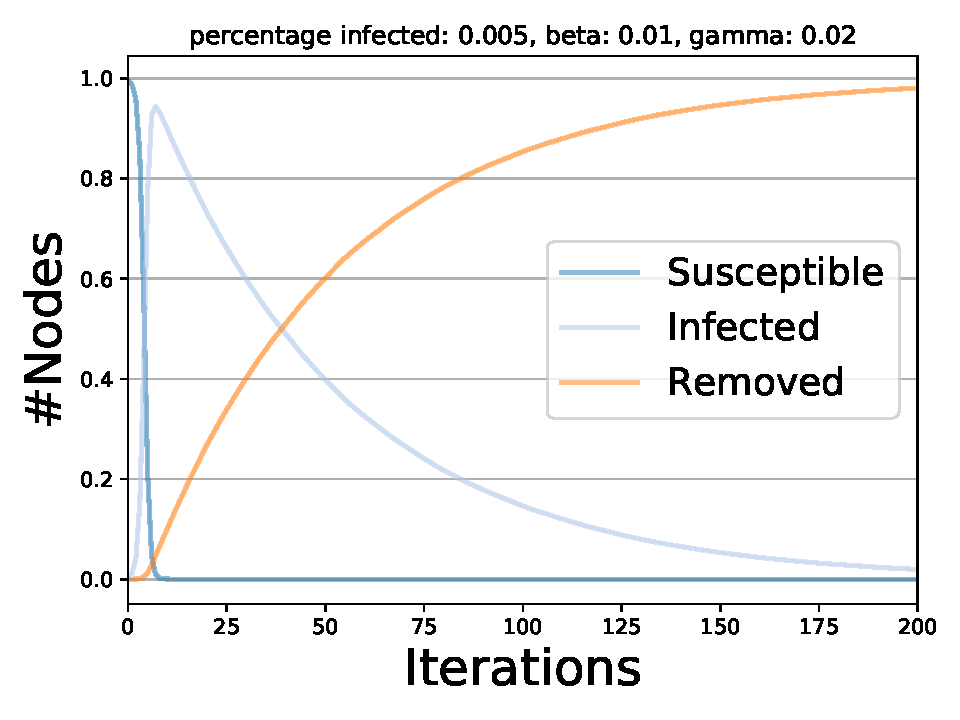
\includegraphics{images/spreading/sir/diffusion_ba_greater.pdf}
            }
            \caption{}
            \label{diff_sir_ba_greater}
        \end{subfigure}
        \caption{In Figure \ref{diff_sir_smaller} and \ref{diff_sir_greater} we can see the representation of the
        diffusion on the original network both for the case in which $\gamma$ is smaller than $\beta$ and the other
        way around. The same kind of representation is plotted for the Erdős–Rényi network in Figure
        \ref{diff_sir_er_smaller} and \ref{diff_sir_er_greater} and for the Barabási–Albert network in Figure
        \ref{diff_sir_ba_smaller} and \ref{diff_sir_ba_greater}.}
        \label{diff_sir_total}
    \end{figure}

% section sir_model (end)

\section{Threshold model} % (fold)
\label{sec:threshold_model}
    Finally we describe the application of the \textbf{Threshold model} both on the original network and the
    synthetic ones. In order to test this model we've choosen to apply a threshold $\tau$ eguals to $0.10$, the
    diffusion of the infection for this model is represented in Figure \ref{diff_thr_total}. As we can see, for the
    original network we have that almost all the nodes become infected within the first $20$ model's iterations,
    due to the fact that the value choosen for the threshold results to be sufficient for the spreading of the
    infection. If we change the threshold's value, this time using $0.20$, we can observe that the
    original network become immune to the infection, thanks to its internal structure. We can observe
    the same immunity in the Erdős–Rényi and Barabási–Albert network for the original threshold's value.
    \begin{figure}[H]
        \centering
        \begin{subfigure}{0.33\textwidth}
            \resizebox{\textwidth}{!}{
                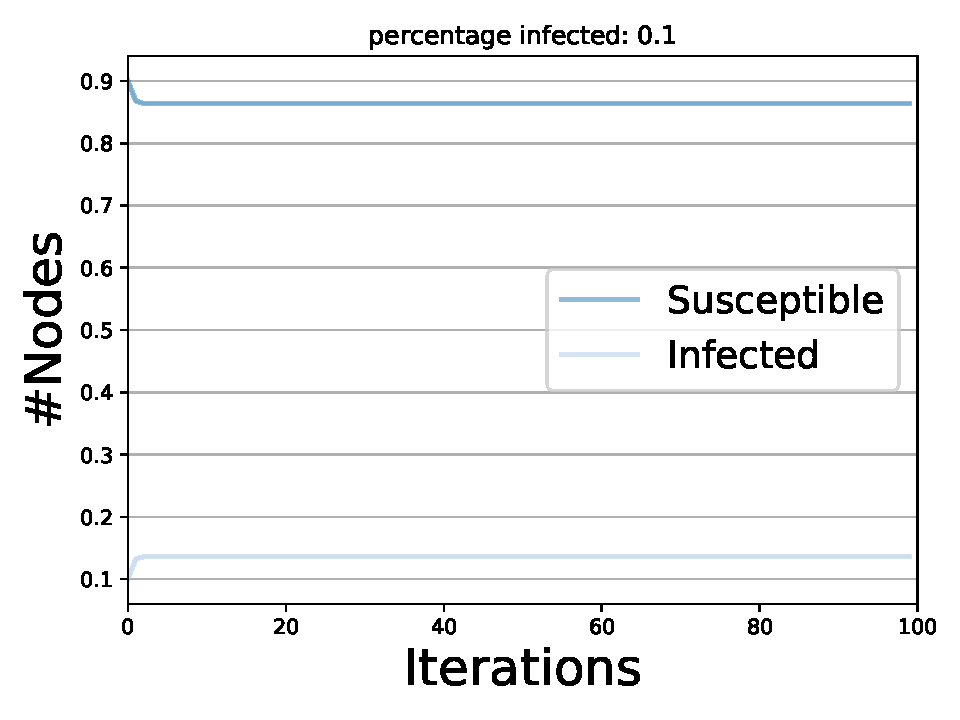
\includegraphics{images/spreading/threshold/diffusion.pdf}
            }
            \caption{}
            \label{diff_thr}
        \end{subfigure}
        \begin{subfigure}{0.33\textwidth}
            \resizebox{\textwidth}{!}{
                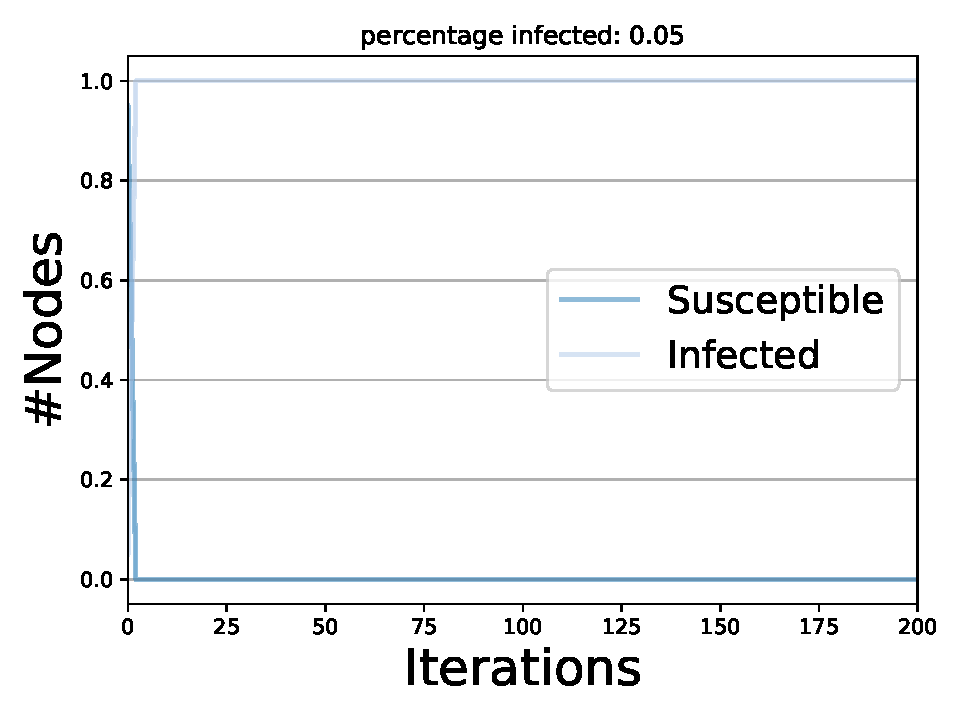
\includegraphics{images/spreading/threshold/diffusion_er.pdf}
            }
            \caption{}
            \label{diff_thr_er}
        \end{subfigure}
        \begin{subfigure}{0.33\textwidth}
            \resizebox{\textwidth}{!}{
                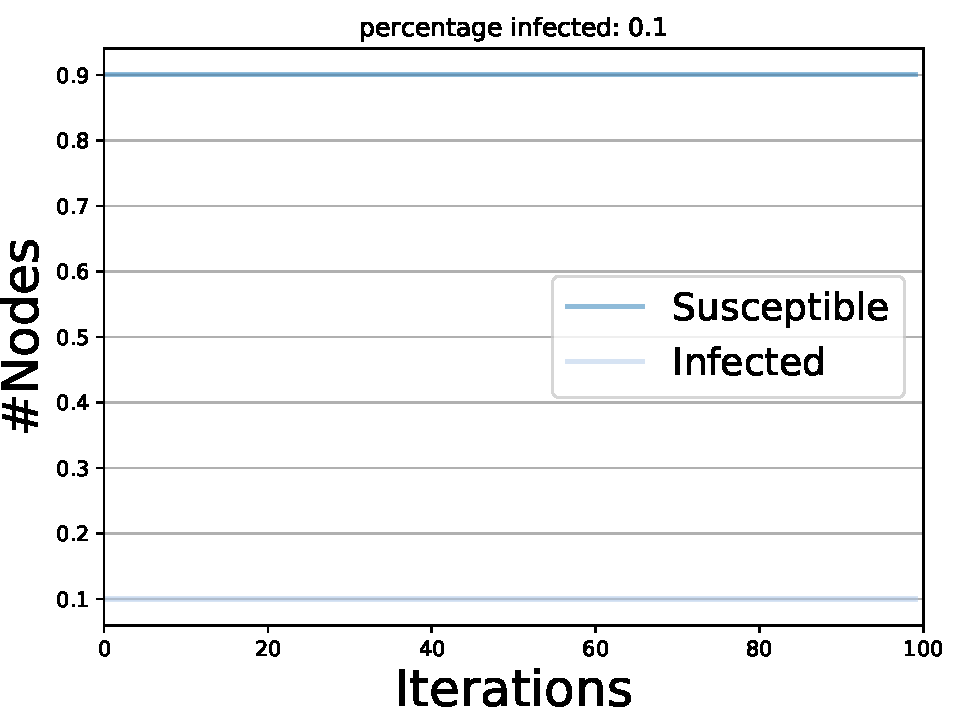
\includegraphics{images/spreading/threshold/diffusion_ba.pdf}
            }
            \caption{}
            \label{diff_thr_ba}
        \end{subfigure}
        \begin{subfigure}{0.33\textwidth}
            \resizebox{\textwidth}{!}{
                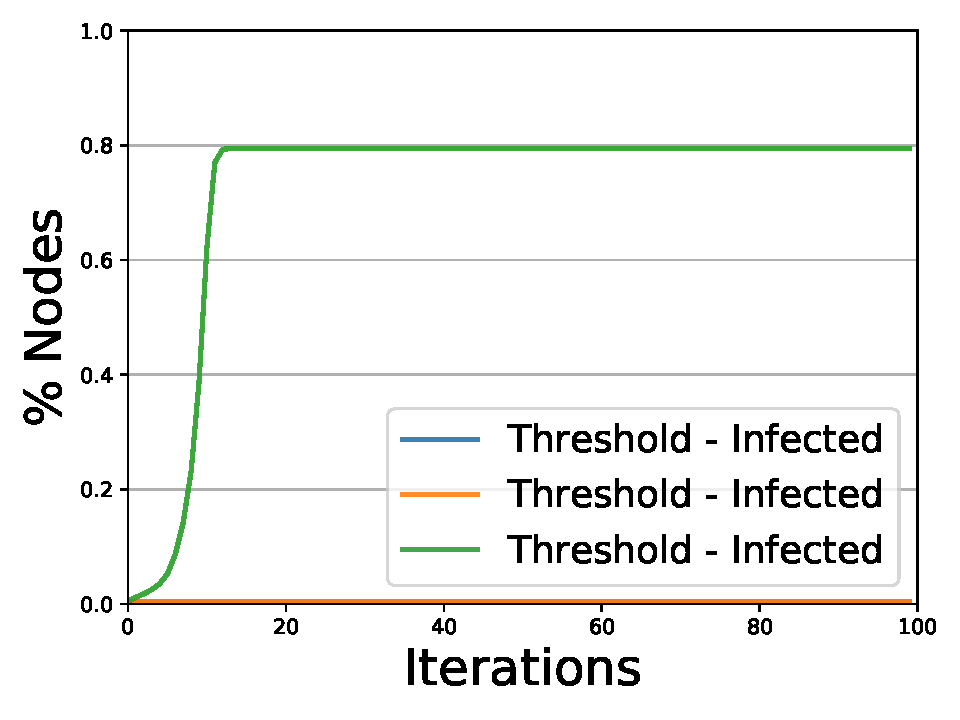
\includegraphics{images/spreading/threshold/trend_comparison.pdf}
            }
            \caption{}
            \label{diff_thr_comparison}
        \end{subfigure}
        \caption{In Figure \ref{diff_thr} is represented the diffusion of the infection for the original network,
        while in Figure \ref{diff_thr_er} and \ref{diff_thr_ba} are represented the cases for the Erdős–Rényi and
        the Barabási–Albert network, respectively. A comparison between the three networks is represented in Figure
        \ref{diff_thr_comparison}.}
        \label{diff_thr_total}
    \end{figure}

% section threshold_model (end)

% chapter spreading (end)
